% f2015zjl_q08_fold.tex — 2015 年高考数学·浙江卷·理科 第 8 题（三角形翻折）
%
% 【来源】`.work/phase3-b19/source/2015浙江理.pdf`（SHA-256
%   801150f0a6d440ac967813d264face6d48b6ee9c69cc20f1c9d6b2b38dec2e9f），
%   第 1 页（合订本页 989）；内容对象 5。逐路径实测见
%   `.work/phase3-b19/figure-inventory.md`。
%
% 【坐标口径】源 PDF 用户空间（原点左下、y 向上）。本图本地坐标
%   (x, y) = (x_page − 532.163, y_page − 239.328)，1 单位 = 1 TeX pt。
%   路径坐标逐点照录内容流（含三次贝塞尔控制点）。
%
% 元素计数：5 条路径（△BDC、A′D、A′C 实线；AD、AC 虚线）＋5 个标签
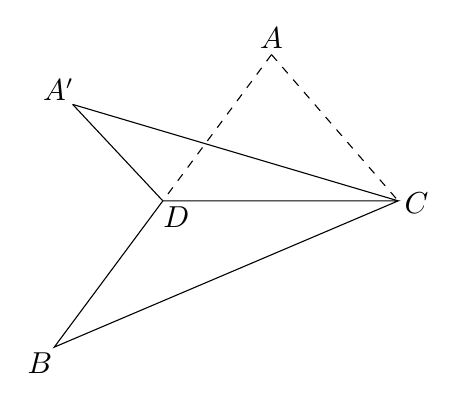
\begin{tikzpicture}[x=1pt, y=1pt,
    every node/.style={inner sep=0pt, font=\fontsize{10.5pt}{12.6pt}\selectfont}]
  \draw[line width=0.398pt] (39.2600,52.8670)   -- (0.0000,0.0000)   -- (124.3000,52.8670)   -- (39.2600,52.8670);
  \draw[line width=0.398pt] (6.6611,87.7336)   -- (39.2601,52.8666);
  \draw[line width=0.398pt] (6.6611,87.7336)   -- (124.3001,52.8666);
  \draw[line width=0.398pt, dash pattern=on 2.989pt off 2.989pt, dash phase=0.0pt] (78.5204,105.7337)   -- (39.2604,52.8667);
  \draw[line width=0.398pt, dash pattern=on 2.989pt off 2.989pt, dash phase=0.0pt] (78.5204,105.7337)   -- (124.3004,52.8667);

  \node[anchor=center] at (78.487,111.712) {$A$};  % 源中心 (610.65,351.04)
  \node[anchor=center] at (1.487,93.012) {$A'$};  % 源中心 (533.65,332.34)
  \node[anchor=center] at (130.887,51.912) {$C$};  % 源中心 (663.05,291.24)
  \node[anchor=center] at (44.087,46.962) {$D$};  % 源中心 (576.25,286.29)
  \node[anchor=center] at (-5.163,-5.888) {$B$};  % 源中心 (527.00,233.44)

\end{tikzpicture}
%
% 【自验结果】
%   探针：latexmk -pdfxe（待跑）。
